\documentclass[aspectratio=169]{beamer}
\usetheme{Madrid}
\usecolortheme{beaver}

\usepackage[UTF8,fontset=fandol]{ctex}
\usepackage{amsmath, amssymb}
\usepackage{booktabs}
\usepackage{ragged2e}
\usepackage{array}
\usepackage{graphicx}
\usepackage{tikz}
\usetikzlibrary{positioning, arrows.meta, shapes.geometric, calc, fit}

\newcommand{\framebottomnote}[1]{%
    \vfill
    \par\noindent
    {\tiny\color{black!65}\parbox{0.96\linewidth}{#1}\par}%
    \vspace*{-0.75cm}%
}

\newcolumntype{L}[1]{>{\RaggedRight\arraybackslash}p{#1}}

\title[0416 进展汇报]{0416 进展汇报}
\subtitle{}
\date{2026-04-16}

\begin{document}

\begin{frame}
    \titlepage
\end{frame}

% ============================================================
\section{机制更新}
% ============================================================

\begin{frame}{最近修改}
\begin{columns}[T]
\begin{column}{0.50\textwidth}
\textbf{前两周的修改}
\begin{itemize}
    \item 任务结果不再直接主导 helplessness
    \item helplessness更新的核心为事件的不可控感 \textbf{uncontrollability}
    \item \textbf{self-efficacy / felt control} 作为中间层或判断层
    \item \textbf{controllable success memory} 提供长期保护
    \item \textbf{support} 不再直接减 helplessness，而是经中间层间接起作用
\end{itemize}
\end{column}

\begin{column}{0.46\textwidth}
\textbf{本周新增的模块Attribution}
\begin{itemize}
    \item 主要解释：
    \begin{itemize}
        \item 为什么负面体验会持续
        \item 为什么会从单任务扩散到任务家族
    \end{itemize}
\end{itemize}
\end{column}
\end{columns}

\end{frame}

\begin{frame}{当前机制主线}
\centering
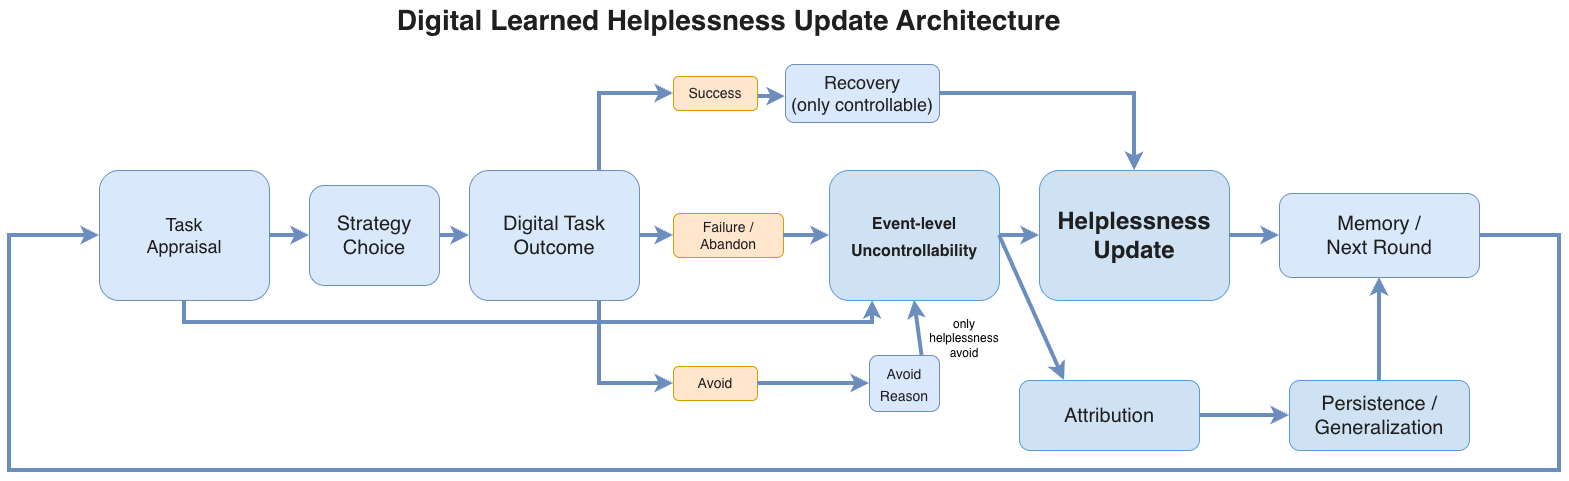
\includegraphics[width=0.96\linewidth,height=0.78\textheight,keepaspectratio]{helplessness_update_architecture.drawio.drawio.drawio.png}

\end{frame}

\begin{frame}[t]{机制依据 I：不可控体验与中间层}
\tiny
\justifying
\textbf{失败与 helplessness 的关系}

数字摩擦的失败不应该直接提升 helplessness，而是先拉低效能感和控制感，再把人推向无助。

\vspace{0.15cm}
\textbf{self-efficacy / felt control 的位置}

把自我效能感和自我的控制感放在agent的判断层中（这个还有待考虑到底怎么建模和放置），低效能、低控制感应当放大负面事件对 helplessness的增幅，而相反的高效能、高控制感会起缓冲作用。

在代码中效能感和控制感也就是作为联系失败和helplessness的中间层。

\vspace{0.18cm}
\textbf{文献支持}

Bandura, A. 1977. Self-Efficacy: Toward a Unifying Theory of Behavioral Change.

An, J., Zhu, X., Wan, K., Xiang, Z., Shi, Z., An, J., et al. 2024. Older Adults' Self-Perception, Technology Anxiety, and Intention to Use Digital Public Services.（这篇主要是tech anxiety，但我感觉好像也差不多)

Sun, Y., Zhang, R., Hu, D., Wang, Y., Wen, C., et al. 2025. Factors That Influence Technophobia in Chinese Older Patients With Ischemic Stroke: A Cross-Sectional Survey.(技术恐惧)

Song, X., Li, S., Dong, L., Li, Y., Yang, X., Bao, J., Liao, S., Xi, Y., and Guo, G. 2025. Technophobia in Digital Health Contexts: A Systematic Review and Meta-Analysis With a Focus on Older Adults(恐惧）
\end{frame}

\begin{frame}[t]{机制依据 II：回避分型与可控成功记忆}
\tiny
\justifying
\textbf{区分不同回避原因}

老人不做/回避数字行为的原因需要区分，不全因为无助，也有怕风险和觉得无用等因素。

把事件结果的avoid分成 \texttt{helpless\_avoid}， \texttt{risk\_avoid} 和 \texttt{low\_value\_avoid}。

只有因为无助而产生的回避才应该显著推高 helplessness，并影响memory。

\vspace{0.12cm}
\textbf{文献支持}

Davis, F. D. 1989. Perceived Usefulness, Perceived Ease of Use, and User Acceptance of Information Technology.

Venkatesh, V., Morris, M. G., Davis, G. B., and Davis, F. D. 2003. User Acceptance of Information Technology: Toward a Unified View.

Jokisch, M. R., Schmidt, L. I., and Doh, M. 2022. Acceptance of Digital Health Services Among Older Adults: Findings on Perceived Usefulness, Self-Efficacy, Privacy Concerns, ICT Knowledge, and Support Seeking.

\vspace{0.16cm}
\textbf{可控成功记忆}

区分出老人真正依靠自己做成、而且感到可控的数字事件。这种事件才会形成长期的对于无助的抵抗，而不是简单的成功次数越多越好。

增加对于可控成功的记忆。

只有agent真正自己学会了、并且觉得这件事是自己能掌控的，才在以后更不容易陷入无助。

如果在support中是被别人完全帮着做完、自己并没有真正掌握的，对于无助的抵抗度应该比前者更低。

\vspace{0.12cm}
\textbf{文献支持}

Niu, H.-J., Li, M.-H., Hsieh, F.-Y., Yu, C.-C., and Lin, C.-T. 2026. From Digital Anxiety to Empowerment in Older Adults: Cross-Sectional Survey Study on Psychosocial Drivers of Digital Literacy.

Lu, S. Y., Yoon, S., Yee, W. Q., Ngiam, N. H. W., Ng, K. Y. Y., and Low, L. L. 2024. Experiences of a Community-Based Digital Intervention Among Older People Living in a Low-Income Neighborhood: Qualitative Study.
\end{frame}

\begin{frame}[t]{机制依据 III：support 路径与 Attribution}
\tiny
\justifying
\textbf{support 的作用方式}

support不应该直接降低helplessness，而是通过提高效能感和控制感等中间层来影响helplessness。

support应该作用到自我效能、可控感这类中间层，再间接影响 helplessness。

\vspace{0.12cm}
\textbf{文献支持}

Zhu, Y., Wang, X., Zhang, X., Li, Y., and Chen, Y. 2025. The Mechanism of Digital Feedback on Health Information Anxiety Among Older Adults: Information Processing Self-Efficacy as a Mediating Variable.

Emmesjö, L., Hallgren, J., and Gillsjö, C. 2025. Older Adults' Digital Technology Experiences: A Qualitative Study.

Jokisch, M. R., Schmidt, L. I., and Doh, M. 2022. Acceptance of Digital Health Services Among Older Adults: Findings on Perceived Usefulness, Self-Efficacy, Privacy Concerns, ICT Knowledge, and Support Seeking.

\vspace{0.16cm}
\textbf{Attribution 扩展层}

人类范畴的习得性无助不应该简化为简单的失败+不可控感，而更应该是人类个体如何解释这种行为与结果之间的非关联性。

区分为 stability、locus 和 scope。

locus(对当前行为和结果非关联性的原因归于 self、situation 还是 mixed)影响自尊自信。

stability（是否认为这种失败的不可控和非关联性在未来仍会持续)进入记忆影响后续 helplessness 的更新和修复强度，以及每次对于事件的预期。

scope(是否将当前任务的失败扩展到所有相似任务)影响 helplessness 的在任务类型的覆盖范围和泛化。

\vspace{0.12cm}
\textbf{文献支持}

Abramson, L. Y., Seligman, M. E. P., and Teasdale, J. D. 1978. Learned Helplessness in Humans: Critique and Reformulation.
\end{frame}

\begin{frame}{Attribution 模块：作用、维度与触发边界}
\begin{columns}[T]
\begin{column}{0.47\textwidth}
\textbf{主要解释}
\begin{itemize}
    \item \textbf{stability}：暂时还是持续
    \item \textbf{scope}：单任务还是任务家族泛化
\end{itemize}
\end{column}

\begin{column}{0.49\textwidth}
\textbf{当前触发边界}
\begin{itemize}
    \item 仅对负向且已尝试过的事件触发：
    \begin{itemize}
        \item \texttt{failure\_after\_attempt}
        \item \texttt{failure\_even\_with\_help}
        \item \texttt{abandon\_midway}
    \end{itemize}
\end{itemize}
\end{column}
\end{columns}

\vspace{0.25cm}
\centering
\scriptsize
\begin{tabular}{lcc}
\toprule
\textbf{维度} & \textbf{正向解释} & \textbf{负向解释} \\
\midrule
Stability & transient & stable \\
Scope & task-specific & family-generalizing \\
\bottomrule
\end{tabular}

\vspace{0.18cm}

{\tiny 当前暂时没把 \textbf{locus} 相关加入主路径中，因为它更偏向自责/情境归因；在还没建模相关状态前，先只做记录。}

\end{frame}

% ============================================================
\section{实验设置与结果}
% ============================================================

\begin{frame}{实验设置}
\textbf{运行配置}
\vspace{0.25cm}
\begin{itemize}
    \item 3 paired seeds: 101 / 201 / 301
    \item 10 agents per world
    \item 7 days
    \item single steady stage
    \item 30-minute logical clock
\end{itemize}

\end{frame}

\begin{frame}[t]{World-Level Results Snapshot}
\centering
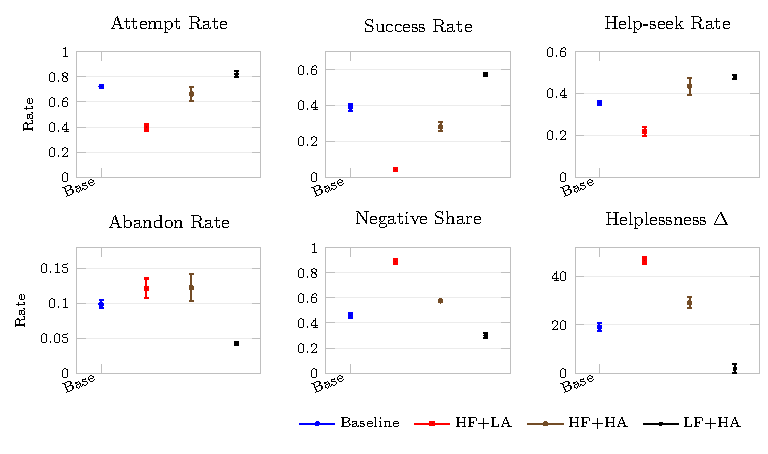
\includegraphics[width=0.82\linewidth,height=0.64\textheight,keepaspectratio]{world_outcomes_facets.pdf}

\vspace{0.15cm}
{\small 新机制下，不同 world 已能稳定拉开行为结果和心理结果}

\framebottomnote{图中误差线为 3 个 paired seeds 的 mean $\pm$ SD。}
\end{frame}

\begin{frame}{Paired Effects vs Baseline}
\centering
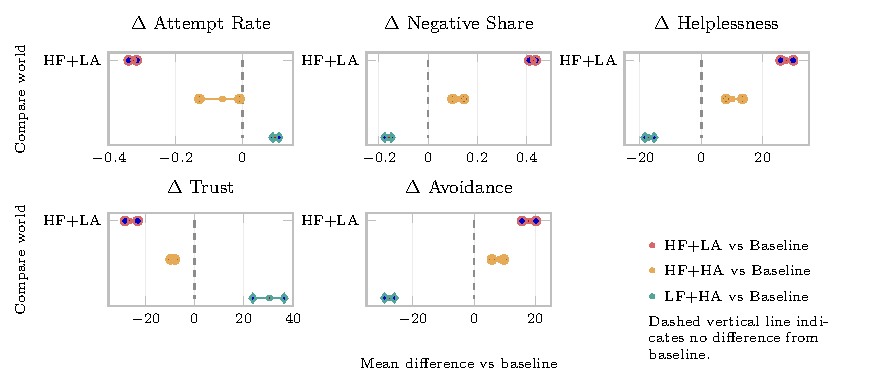
\includegraphics[width=0.95\linewidth]{world_paired_effects_forest.pdf}
\end{frame}

\begin{frame}[t]{Attribution Results Across Worlds}
\begin{columns}[T]
\begin{column}{0.30\textwidth}
\vspace{0.55cm}
\small
\textbf{坏环境不仅提高失败率，\\也改变失败解释的方式}
\end{column}

\begin{column}{0.68\textwidth}
\centering
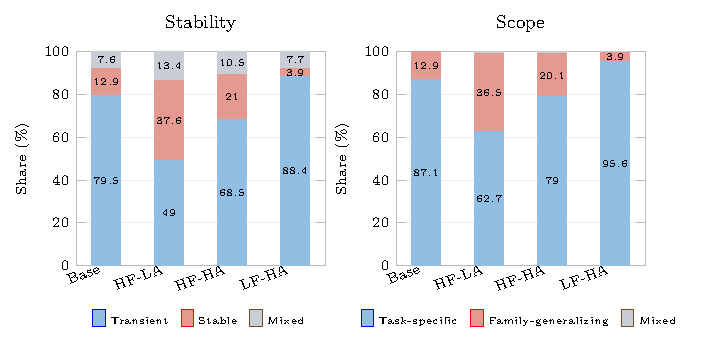
\includegraphics[width=\linewidth]{attribution_worlds_paper.pdf}
\end{column}
\end{columns}

\end{frame}

% ============================================================
\section{总结}
% ============================================================

\begin{frame}{本周结论与下一步}
\begin{columns}[T]
\begin{column}{0.48\textwidth}
\textbf{本周结论}
\begin{itemize}
    \item helplessness update 已经从原本简单的失败累积进一步改进到不可控体验驱动
    \item attribution 模块已成功接入，并能跑出分化
    \item 新实验结果整体支持当前机制方向
\end{itemize}
\end{column}

\begin{column}{0.48\textwidth}
\textbf{下一步}
\begin{itemize}
    \item 补更多 seeds，提升结果稳定性
    \item 继续收紧机制复杂度与论文叙事
    \item 考虑消融实验
\end{itemize}
\end{column}
\end{columns}

\end{frame}

\begin{frame}
    \centering
    \Huge{请老师批评指正}
\end{frame}

\end{document}
